\documentclass[12pt]{article}  % 官方要求字号不小于 12 号,此处选择 12 号字体
% \linespread{1.1}
% \bibliographystyle{plain}
% 本模板不需要填写年份,以当前电脑时间自动生成
% 请在以下的方括号中填写队伍控制号
\usepackage[]{easymcm}  % 载入 EasyMCM 模板文件
\usepackage{palatino}  
\usepackage{pdfpages}
\usepackage{longtable}
\usepackage{tabu}
\usepackage{threeparttable}
\usepackage{listings}
\usepackage{paralist}
\usepackage{setspace}
\usepackage{CJKutf8}
\usepackage{textcomp} % 必须加上,否则报错
\usepackage[framed,numbered,autolinebreaks,useliterate]{mcode}    % 添加matlab代码宏

\let\itemize\compactitem
\let\enditemize\endcompactitem
\newcommand{\upcite}[1]{\textsuperscript{\textsuperscript{\cite{#1}}}}

\title{摘要} 

% 文档开始
\begin{document}
\begin{abstract}
	\vspace{15pt}
	本项目的核心任务是通过统计过程控制(SPC)方法,对某工厂生产的滚珠直径数据进行产品质量管理,评估产品工艺水平及其生产过程是否受控。统计过程控制作为一种基于概率统计的过程控制方法,自1924年由Shewhart博士提出控制图以来,已广泛应用于现代制造过程的质量控制中。本项目基于Matlab软件开发,对于收集到的数据,通过描述性统计分析、正态性检验、总体均值检验、工序能力指数计算与绘制均值控制图和方差控制图等多种方式,对数据进行全面分析,最终评估工艺水平及生产过程的受控状态。具体而言,首先,在数据收集过程中,结合实际数据与模拟数据,得到25组产品质量样本数据(每组至少5个样本);随后,通过描述性统计分析方法对数据进行宏观的认知,根据均值、方差、极差、直方图等指标对数据进行初步分析;接着又利用假设检验的方法,分别通过Pearson卡方检验与t检验等方法验证数据是否符合正态分布,并对其总体均值进行检验。基于对于正态总体及其均值、方差的检验合理性,最终计算并评估了数据的工序能力指数,同时绘制了均值控制图和方差控制图,以直观反映生产过程中的数据波动情况。通过多种方法的综合分析,最终得出了工厂生产的滚珠直径的工艺水平评价和生产过程的受控状态判断。
	\vspace{5pt}
	\noindent
	
	\textbf{关键词}: 产品质量管理、统计过程控制(SPC)、假设检验、Shewhart控制图、Matlab
\end{abstract}

\maketitle  

\tableofcontents

\section{项目概述}

\subsection{问题背景}
现代产品质量管理主要有两个核心目标:第一,评价产品的工艺水平如何,即产品质量如何;第二,评价产品的生产过程是否受控,即产品可靠性如何。从现代质量控制的角度看,一方面要求产品质量好,另一方面还要求可靠性高。	

统计过程控制(Statistical Process Control, SPC)是一种基于概率统计的过程控制方法。1924年美国贝尔实验室的Shewhart博士提出控制图,标志着产品统计质量控制的正式起点。作为现代质量管理的重要方法,SPC广泛应用于现代制造过程的质量控制。20实际80年代,国际上半导体制造过程已经普遍采用SPC技术提升产品合格率和可靠性。比如Motorola公司提出并在美国通用电器公司等广泛应用的$6\sigma$管理,其主要技术基础就是SPC理论。	

生产过程是否处于统计受控状态,取决于生产过程是否存在异常因素导致产品质量的起伏变化。产品加工结果是否满足加工规范要求,反应的是工艺水平的高低;而工艺是否受控,反应的是生产过程是否存在异常因素。

\subsection{项目任务}	
在本次项目中,需要收集批量产品质量数据,利用SPC方法对其进行管理,分析整体工艺水平并判断生产过程是否处于统计受控状态,具体而言可细分为如下任务:
\begin{itemize}
	\setlength{\parsep}{0ex} %段落间距
	\setlength{\topsep}{2ex} %列表到上下文的垂直距离
	\setlength{\itemsep}{1ex} %条目间距
	\item \textbf{任务 1}:收集或生成25组以上的数据,每组至少5个样本。		
	\item \textbf{任务 2}:根据均值,方差,极差,直方图等指标,对数据进行描述性统计分析。
	\item \textbf{任务 3}:对数据进行正态性检验与总体的均值检验。
	\item \textbf{任务 4}:计算数据工序能力指数并对其进行评估。
	\item \textbf{任务 5}:描绘均值控制图和方差控制图。
	\item \textbf{任务 6}:得出结论:工艺水平如何;生产过程是否处于统计受控状态。
\end{itemize}

\section{项目过程}
本项目完全基于Matlab代码实现SPC方法进行产品质量管理。
\subsection{数据收集}
本项目中的数据收集采用实际数据与模拟数据结合的方式,其中实际数据以书本7.4节的例题7.4.4\upcite{1}为主要来源,在此基础上利用生成的模拟数据对其进行扩充,最终得到25组产品质量样本数据,每组中含有5个数据。

具体而言,本项目的问题情境为对工厂生产的滚珠直径(单位:$mm$)进行产品质量管理。书本上的例题提供了50个直径数据,将其作为扩充生成模拟数据的源数据$source\_data$,即:
\begin{lstlisting}
source_data=[15.0,15.8,15.2,15.1,15.9,
			 14.7,14.8,15.5,15.6,15.3,
			 15.0,15.6,15.7,15.8,14.5,
			 15.1,15.3,14.9,14.9,15.2,
			 15.9,15.0,15.3,15.6,15.1,
			 14.9,14.2,14.6,15.8,15.2,
			 15.2,15.0,14.9,14.8,15.1,
			 15.5,15.5,15.1,15.1,15.0,
			 15.3,14.7,14.5,15.5,15.0,
			 14.7,14.6,14.2,14.2,14.5]; 
\end{lstlisting}

设置扩充后的数据组数$num\_groups$以及各组样本数据个数$samples\_per\_groups$:

\begin{lstlisting}
num_groups = 25;
samples_per_group = 5;
\end{lstlisting}

两者相乘得到样本数据总数$num\_data\_points$:
\begin{lstlisting}
num_data_points = num_groups * samples_per_group;
\end{lstlisting}

要对原始数据进行扩充,首先需要复制原始数据并添加随机扰动:
\begin{lstlisting}
replicated_data = repmat(source_data, 1, ceil(num_data_points / length(source_data)));
perturbed_data = replicated_data(1:num_data_points) + 0.05 * randn(1, num_data_points);
\end{lstlisting}

接着使用插值生成更多数据点,并保留一位小数:
\begin{lstlisting}
x = 1:length(perturbed_data);
xi = linspace(1, length(perturbed_data), num_data_points);
interpolated_data = interp1(x, perturbed_data, xi, 'spline');
interpolated_data = round(interpolated_data, 1);
\end{lstlisting}

最后将生成的模拟数据点重新组织为25组,每组5个数据,得到完整样本数据:
\begin{lstlisting}
expanded_data = reshape(interpolated_data, samples_per_group, num_groups)';
data = expanded_data;
\end{lstlisting}

最终的样本数据如下表所示:
\begin{longtable}[]{@{}llllll@{}}
	\toprule\noalign{}
	& 1 & 2 & 3 & 4 & 5 \\
	\midrule\noalign{}
	\endhead
	\bottomrule\noalign{}
	\endlastfoot

	1 & 15.0000 & 14.6000 & 15.0000 & 15.1000 & 16.0000 \\
	2 & 14.9000 & 15.2000 & 15.5000 & 15.2000 & 14.7000 \\
	3 & 15.7000 & 14.7000 & 15.6000 & 15.2000 & 15.0000 \\
	4 & 14.2000 & 15.1000 & 15.5000 & 14.7000 & 14.6000 \\
	5 & 15.2000 & 15.5000 & 15.7000 & 14.9000 & 15.3000 \\
	6 & 14.7000 & 14.9000 & 15.1000 & 14.4000 & 14.3000 \\
	7 & 15.1000 & 15.6000 & 15.8000 & 14.8000 & 15.6000 \\
	8 & 15.9000 & 14.8000 & 15.1000 & 15.5000 & 14.3000 \\
	9 & 16.0000 & 15.3000 & 14.6000 & 15.3000 & 15.1000 \\
	10 & 15.2000 & 15.1000 & 15.1000 & 14.9000 & 14.6000 \\
	11 & 15.0000 & 14.8000 & 14.9000 & 15.1000 & 15.9000 \\
	12 & 14.9000 & 15.3000 & 15.5000 & 15.2000 & 14.7000 \\
	13 & 15.8000 & 14.8000 & 15.6000 & 15.3000 & 14.9000 \\
	14 & 14.1000 & 15.1000 & 15.4000 & 14.7000 & 14.6000 \\
	15 & 15.2000 & 15.5000 & 15.7000 & 14.9000 & 15.3000 \\
	16 & 14.6000 & 14.9000 & 15.0000 & 14.5000 & 14.3000 \\
	17 & 15.2000 & 15.6000 & 15.8000 & 14.9000 & 15.6000 \\
	18 & 15.8000 & 14.8000 & 15.1000 & 15.5000 & 14.2000 \\
	19 & 15.9000 & 15.3000 & 14.5000 & 15.2000 & 15.1000 \\
	20 & 15.2000 & 15.1000 & 15.0000 & 15.0000 & 14.5000 \\
	21 & 15.0000 & 14.7000 & 15.0000 & 15.1000 & 16.0000 \\
	22 & 14.9000 & 15.1000 & 15.6000 & 15.3000 & 14.6000 \\
	23 & 15.7000 & 14.9000 & 15.6000 & 15.4000 & 14.9000\\
	24 & 14.2000 & 15.0000 & 15.5000 & 14.8000 & 14.7000 \\
	25 & 15.2000 & 15.4000 & 15.6000 & 14.9000 & 15.2000 \\
\end{longtable}
其中每行表示一组数据,共25组,每组中有5个数据。

\subsection{描述性统计分析}
描述性统计量主要有以下几种:

\begin{itemize}
	\setlength{\parsep}{0ex} %段落间距
	\setlength{\topsep}{2ex} %列表到上下文的垂直距离
	\setlength{\itemsep}{1ex} %条目间距
	\item \textbf{均值 (Mean)}: 计算每组数据的平均值,反映该组数据的中心位置。		
	\item \textbf{方差 (Variance)}: 度量数据分散程度,数值越大表示数据的波动越大。
	\item \textbf{标准差 (Standard Deviation)}: 方差的平方根,同样反映数据的分散程度,但单位与数据相同。
	\item \textbf{极差 (Range)}: 最大值与最小值的差,表示数据的跨度。
\end{itemize}

利用Matlab软件中自带的库函数,可以分别实现对于各组数据均值、方差、标准差与极差等统计量的计算:
\begin{lstlisting}
means = mean(data, 2); 
variances = var(data, 0, 2); 
ranges = range(data, 2); 
stds = std(data, 0, 2);
\end{lstlisting}

\begin{longtable}[]{@{}llllll@{}}
	\toprule\noalign{}
	& 各组均值 & 各组方差 & 各组标准差 & 各组极差 \\
	\midrule\noalign{}
	\endhead
	\bottomrule\noalign{}
	\endlastfoot

	1 & 15.14 & 0.268 & 0.51769 & 1.4 \\
	2 & 15.1 & 0.095 & 0.30822 & 0.8 \\
	3 & 15.24 & 0.173 & 0.41593 & 1 \\
	4 & 14.82 & 0.247 & 0.49699 & 1.3 \\
	5 & 15.32 & 0.092 & 0.30332 & 0.8 \\
	6 & 14.68 & 0.112 & 0.33466 & 0.8 \\
	7 & 15.38 & 0.172 & 0.41473 & 1 \\
	8 & 15.12 & 0.382 & 0.61806 & 1.6 \\
	9 & 15.26 & 0.253 & 0.50299 & 1.4 \\
	10 & 14.98 & 0.057 & 0.23875 & 0.6 \\
	11 & 15.14 & 0.193 & 0.43932 & 1.1 \\
	12 & 15.12 & 0.102 & 0.31937 & 0.8 \\
	13 & 15.28 & 0.187 & 0.43243 & 1 \\
	14 & 14.78 & 0.247 & 0.49699 & 1.3 \\
	15 & 15.32 & 0.092 & 0.30332 & 0.8 \\
	16 & 14.66 & 0.083 & 0.2881 & 0.7 \\
	17 & 15.42 & 0.132 & 0.36332 & 0.9 \\
	18 & 15.08 & 0.387 & 0.62209 & 1.6 \\
	19 & 15.2 & 0.25 & 0.5 & 1.4 \\
	20 & 14.96 & 0.073 & 0.27019 & 0.7 \\
	21 & 15.16 & 0.243 & 0.49295 & 1.3 \\
	22 & 15.1 & 0.145 & 0.38079 & 1 \\
	23 & 15.3 & 0.145 & 0.38079 & 0.8 \\
	24 & 14.84 & 0.223 & 0.47223 & 1.3 \\
	25 & 15.26 & 0.068 & 0.26077 & 0.7 \\
\end{longtable}

以及计算总体数据的均值、方差、标准差与极差:
\begin{lstlisting}
overall_mean = mean(data(:)); 
overall_variance = var(data(:)); 
overall_range = range(data(:)); 
overall_std = std(data(:));
\end{lstlisting}

\begin{longtable}[]{@{}llllll@{}}
	\midrule\noalign{}
	\endhead
	\bottomrule\noalign{}
	\endlastfoot

	总体均值 & 15.1064 \\
	总体方差 & 0.18657\\
	总体标准差 & 0.43194\\
	总体极差 & 1.9\\
\end{longtable}

值得注意的是,Matlab中计算方差的函数 var(A) 默认会按照 $N-1$($N$ 是观测值数量,即上文中的$num\_data\_points$)实现归一化,从而可以作为对于总体分布的方差的无偏估计。上述得到的均为修正后的样本方差。

通过对于上述四个描述性统计量的样本观测结果进行初步分析,可以得到如下结论:
\begin{itemize}
	\setlength{\parsep}{0ex} %段落间距
	\setlength{\topsep}{2ex} %列表到上下文的垂直距离
	\setlength{\itemsep}{1ex} %条目间距
	\item 滚珠直径的总体平均值约为15.1mm,可作为后续总体均值检验的检验目标。		
	\item 各组数据的方差均在0.5以内,总体方差与标准差也较低,说明生产过程中数据波动较小,产品质量稳定性较高。
	\item 数据极差范围适中,总体极差不超过2,处于合理区间。
\end{itemize}

除此之外,还可以通过绘制频数分布直方图的方式对于样本数据进行描述性统计分析:
\begin{lstlisting}
h = histogram(data);
\end{lstlisting}

\begin{figure}[H]
	\centering
	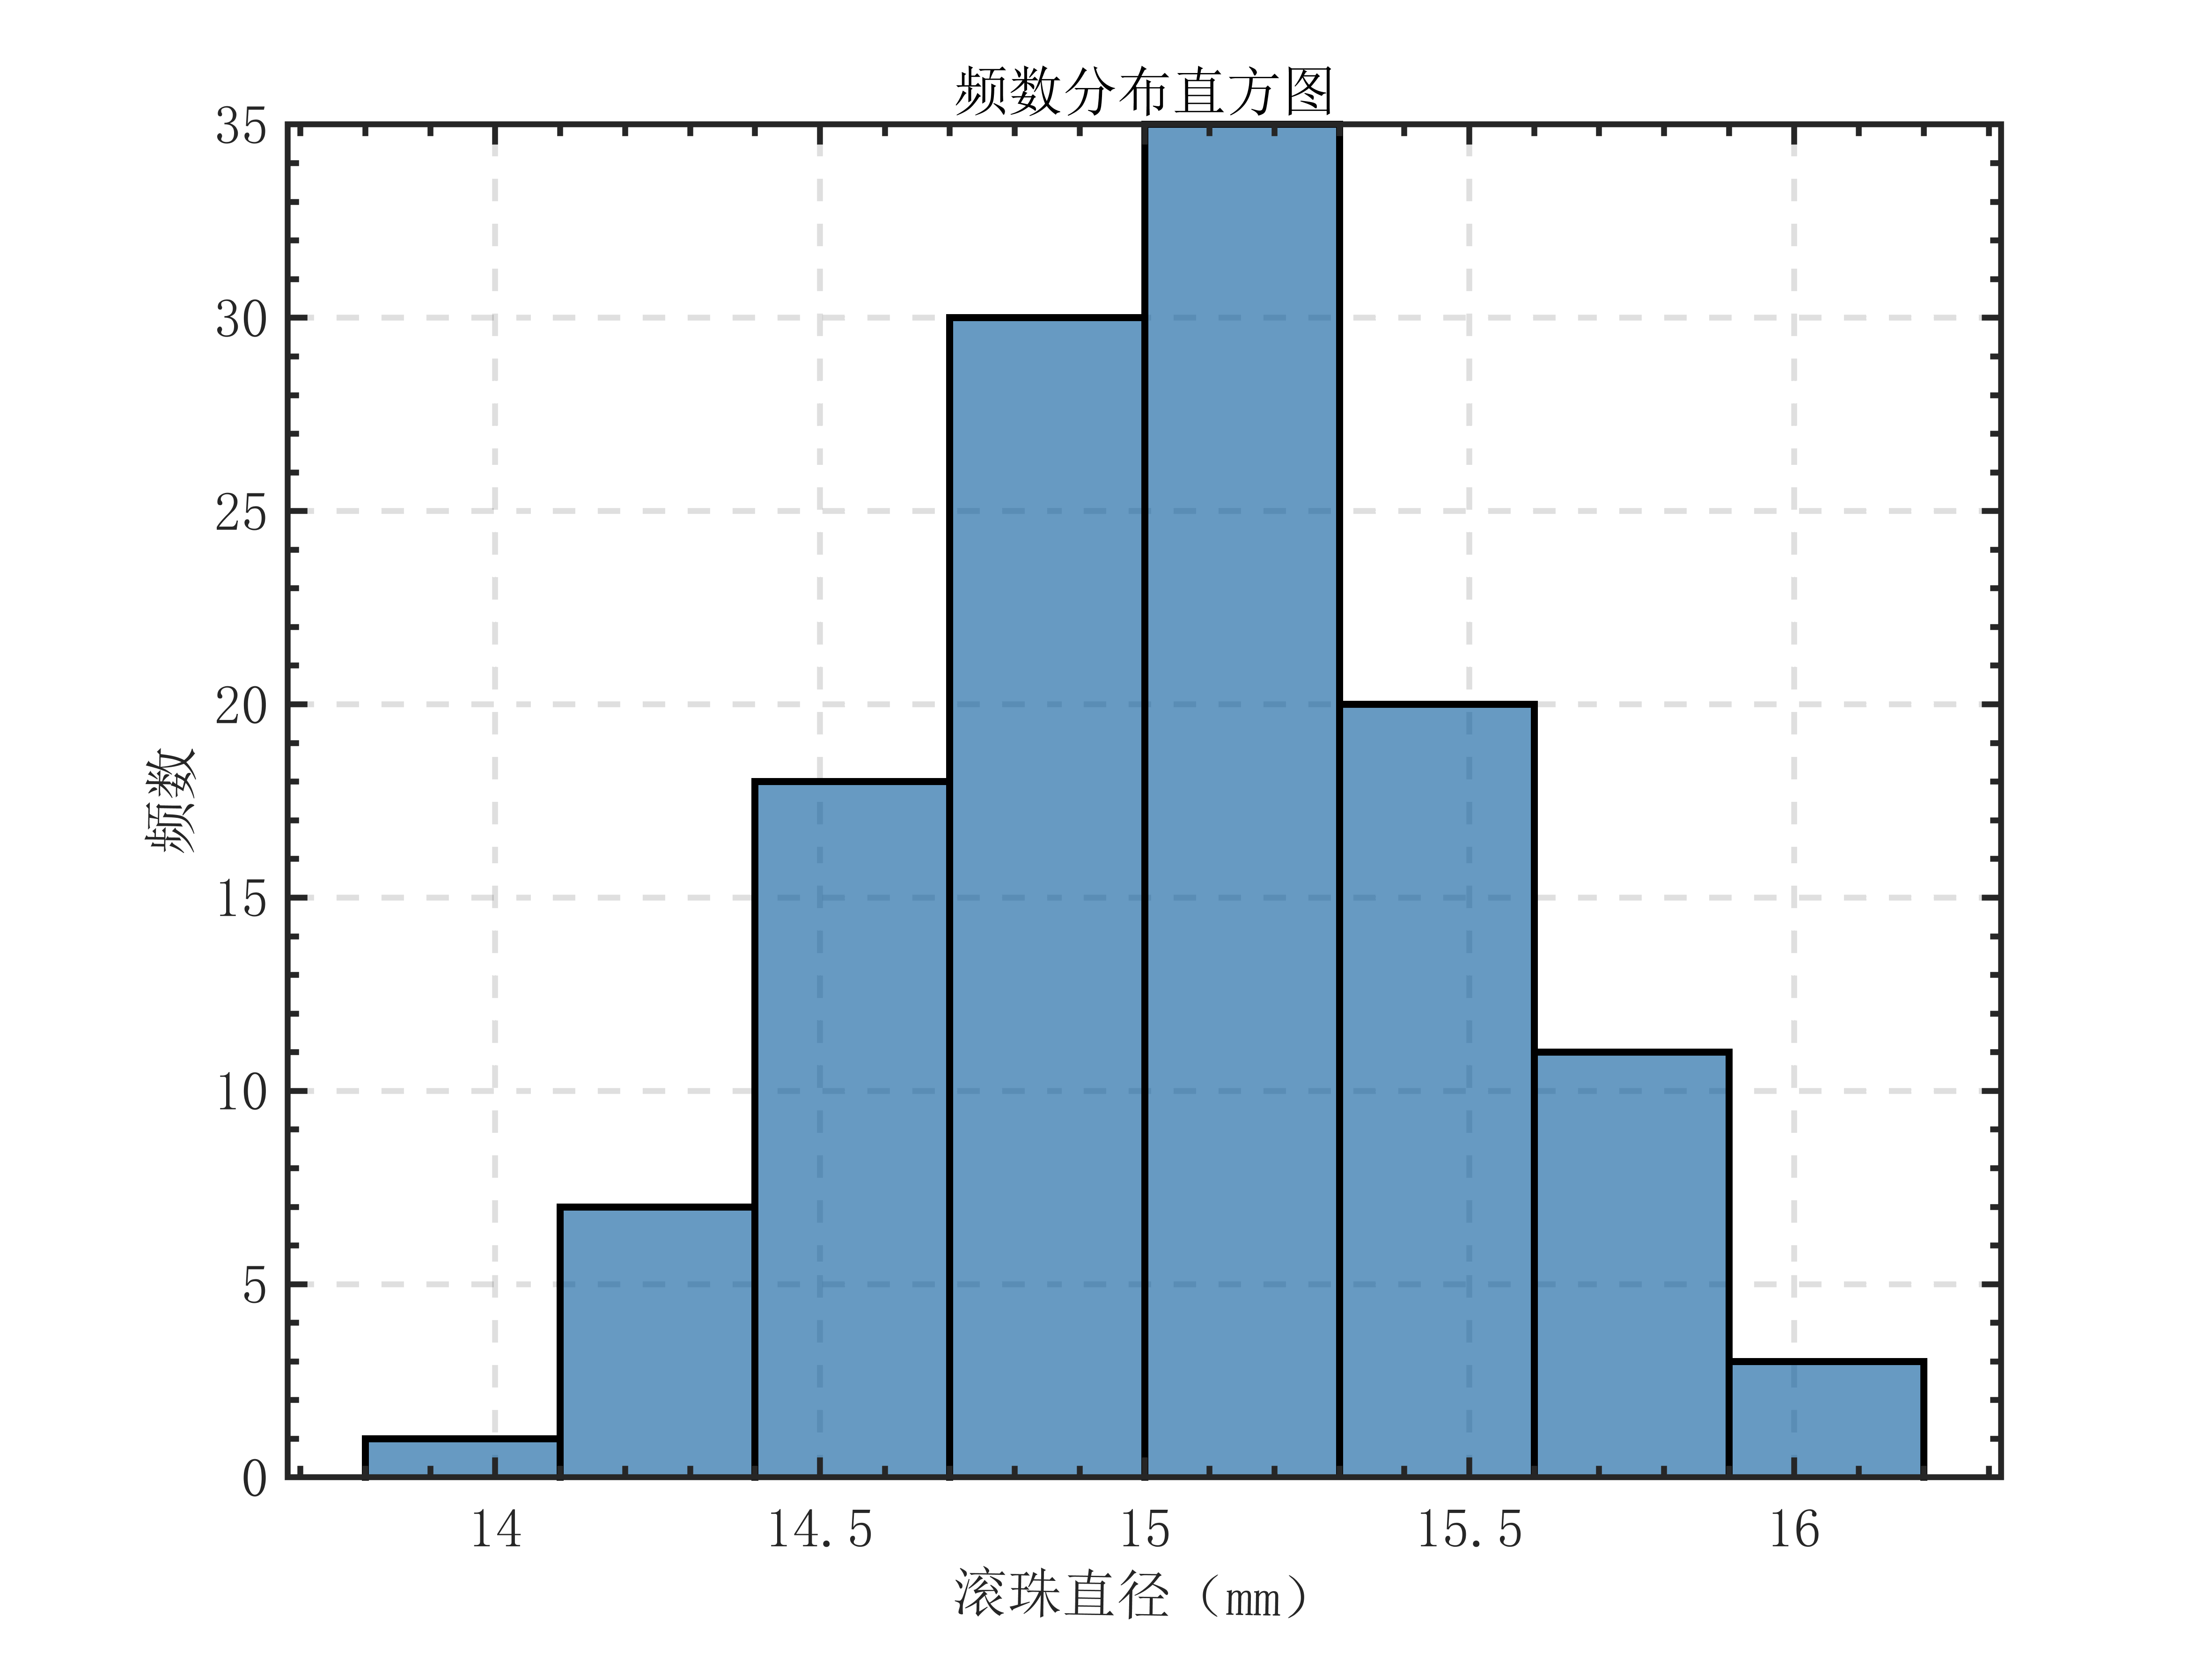
\includegraphics[width=1\textwidth]{1.png}
\end{figure}

观察图表可知,\textbf{数据的频数分布大致呈“两边少,中间多”的趋势,推测其总体大致服从正态分布},需要进行进一步检验。

\subsection{数据正态性检验}
要验证总体是否服从正态分布,需要采用Pearson卡方检验方法,对总体的分布类型进行检验。

Matlab软件中,有相应的函数$chi2gof$可通过Pearson卡方检验来验证总体分布类型是否为正态分布:

\begin{lstlisting}
[result, p_chi2] = chi2gof(data(:));
\end{lstlisting}

$chi2gof$函数是使用Pearson卡方检验返回原假设的检验决策,其原假设假定样本数据来自正态分布的总体,备择假设是样本数据不来自正态分布的总体。默认情况(仅将样本数据$data$输入$chi2gof$函数)下,检验的显著性水平为$\delta=0.05$,且默认检验总体是否服从正态分布;通过增加函数的输入参数可以对显著性水平和检验的分布类型进行更改,在此不再赘述。

返回的参数$result$为正态性检验的结果,若$result=0$,说明无法拒绝原假设,即可认为样本数据来自正态分布的总体;若$result=1$,则拒绝原假设,认为数据不来自正态分布的总体。另一返回参数$p\_chi2$则为该检验的$p$值,当其大于显著性水平$\delta$时不拒绝原假设。

\textbf{通过对样本数据进行正态性检验,可认为数据来自正态分布的总体,正态性检验的$p$值为$0.37005$。}

从原理出发,也可根据假设检验的基本方法流程对总体的分布类型进行检验:

首先,提出原假设与备择假设:
\begin{itemize}
	\setlength{\parsep}{0ex} %段落间距
	\setlength{\topsep}{2ex} %列表到上下文的垂直距离
	\setlength{\itemsep}{1ex} %条目间距
	\item \textbf{$H_0$}:总体服从正态分布,即$F(x) = \phi(\frac{x-\mu}{\sigma})$;		
	\item \textbf{$H_1$}:总体不服从正态分布,即$F(x) \neq \phi(\frac{x-\mu}{\sigma})$。
\end{itemize}

其中$F(x)$为总体的分布,$\mu$和$\sigma$为正态分布的均值与方差(均为未知参数)。

接着,根据假设的提出给出对应的拒绝域形式:$R_0 = \left\{ T>c \right\} $,其中$T$为构造的统计量:

\begin{equation}
	T=\sum_{i=1}^{r}\frac{{{(n_i-np}_i)}^2}{np_i}
\end{equation}

若将对总体$X$所有可能的取值范围分割成$r$个两两不交的部分,则式中:

\begin{itemize}
	\setlength{\parsep}{0ex} %段落间距
	\setlength{\topsep}{2ex} %列表到上下文的垂直距离
	\setlength{\itemsep}{1ex} %条目间距
	\item \textbf{$n_i$}:统计样本中实际落入第$i$个部分的个数(实际频数);		
	\item \textbf{$n$}:样本数据总数,即上文代码中的$num\_data\_points$;
	\item \textbf{$p_i$}:任一样本落入第$i$个部分的概率。
\end{itemize}

显然,当原假设$H_0: F(x) = \phi(\frac{x-\mu}{\sigma})$成立时,理论频数$n*p_i$应与实际频数$n_i$较为接近,这也是拒绝域形式的确定依据。

可以注意到,Pearson卡方统计量$T=\sum_{i=1}^{r}\frac{{{(n_i-np}_i)}^2}{np_i}$服从如下的大样本分布:

\begin{equation}
\hat{T}=\sum_{i=1}^{r}\frac{{{(n_i-n\hat{p}}_i)}^2}{n{\hat{p}}_i}\rightarrow X^2(r-1-s)
\end{equation}

其中:
\begin{itemize}
	\setlength{\parsep}{0ex} %段落间距
	\setlength{\topsep}{2ex} %列表到上下文的垂直距离
	\setlength{\itemsep}{1ex} %条目间距
	\item $s$表示待估未知参数的个数,显然本项目中$s=2$;		
	\item ${\hat{p}}_i$为任一样本落入第$i$部分的概率$p_i$的估计值,这是由于假定的分布类型中含有未知参数,因此需要先根据样本数据对未知参数进行极大似然估计,再代入得到概率的估计值。
\end{itemize}

然后,需要计算犯第一类错误的概率$\alpha=P \left\{H_1|H_0\right\} = \left\{T>c|\\F(x)=F_0(x)\right\}$,并根据$\alpha = \delta = 0.05$求得拒绝域中未知参数$c$的临界值$criticalValue = 11.0705$:

\begin{lstlisting}
deta=0.05;
mu_MLE = overall_mean;
sigma2_MLE = overall_variance*(num_data_points-1)/num_data_points; 
sigma_MLE = sqrt(sigma2_MLE);
dimension=numBins-1-2;
criticalValue = chi2inv(1 - deta, dimension);
\end{lstlisting}

事实上,上文中提到Matlab软件中的var(A)函数默认按照$N-1$实现归一化,而正态分布方差的极大似然估计应为未修正的样本方差,故特此进行更正;同时,在2.2节的描述性统计分析过程中,涉及到频数直方图的绘制时已经对数据完成了分组,可直接通过读取上述的图表属性获取分组数$numBins$(对应上文中$r$)、各组频数$binCounts$(对应上文中实际频数$n_i$与各分组边界$binEdges$(可用于计算$p_i$)):

\begin{lstlisting}
numBins = h.NumBins;
binCounts = h.Values;
binEdges = h.BinEdges;
\end{lstlisting}

最后,通过样本数据计算出对应卡方统计量$T$的观测值$kafang = 2.6897$:
\begin{lstlisting}
kafang=0;
p_hat(1)= normcdf(binEdges(2), mu_MLE, sigma_MLE);
for i=2:numBins-1
	p_hat(i)= normcdf(binEdges(i+1), mu_MLE, sigma_MLE)-normcdf(binEdges(i), mu_MLE, sigma_MLE);
end
p_hat(numBins)= 1-normcdf(binEdges(numBins), mu_MLE, sigma_MLE);
for i=1:numBins
	kafang=kafang+(binCounts(i)-num_data_points*p_hat(i))^2 / (num_data_points*p_hat(i));
end
\end{lstlisting}

\textbf{由于$ kafang<criticalValue $,即不位于拒绝域内,因此无法拒绝原假设$H_0$,即可以认为数据确实来自正态分布的总体},与直接调用Matlab内置库函数的结果一致。

\subsection{总体均值检验}
通过Pearson卡方检验,已经可以认为在显著性水平$\delta=0.05$的情况下,总体近似服从正态分布。进一步地,还希望对该正态总体的均值参数$\mu$进行假设检验。在2.2节的描述性统计分析过程中,已经计算得到样本的总体均值(实际上也是正态分布参数$\mu$的无偏估计与最大似然估计)$\mu_0$ 约为15.1(mm),因此接下来的假设检验过程就将其作为检验对象:

\begin{lstlisting}
miu0=15.1;
\end{lstlisting}

在正态总体的均值检验过程中,主要采取t检验的方法,即认为正态总体的另一参数$\sigma$未知。这样的检验方法的合理性是显然的,此时需要构造服从t分布的统计量以进行t检验。

在Matlab软件中,对于t检验仍然有相对应的库函数$ttest()$可以调用:

\begin{lstlisting}
[result1, ttest_p_value] = ttest(data(:),miu0);
\end{lstlisting}

函数$ttest(data(:),miu0)$使用单样本t检验返回原假设的检验决策,其原假设假定数据$data$来自均值等于输入参数$miu0$且方差未知的正态分布,而备择假设是总体分布的均值不等于$miu0$。如果该检验在默认为$5\%$的显著性水平上拒绝原假设,则函数的返回值$result1$为1,即认为正态总体的均值不为$miu0$,否则为0;而另一返回值$ttest\_p\_value$则为该检验的$p$值,当其大于显著性水平时不拒绝原假设,即可认为正态总体的均值等于$miu0$。

运行代码可得:\textbf{正态总体均值检验$p$值$ttest\_p\_value=0.8687$,可认为正态总体的均值约为$\mu_0=15.1$。}

同样的,这样的假设检验过程也可以基于一般的统计方法实现:

首先,提出原假设与备择假设:
\begin{itemize}
	\setlength{\parsep}{0ex} %段落间距
	\setlength{\topsep}{2ex} %列表到上下文的垂直距离
	\setlength{\itemsep}{1ex} %条目间距
	\item \textbf{$H_0$}:正态总体的均值为15.1,即$\mu=\mu_0=15.1$;		
	\item \textbf{$H_1$}:正态总体的均值不为15.1,即$\mu \neq \mu_0$。
\end{itemize}

接着,根据假设的提出给出对应的拒绝域形式:$R_0 = \left\{ (x_1, x_2,...,x_n)^T :|\bar{x}-\mu_0| >c \right\} $。
该拒绝域形式的构造是具有合理性的,因为显然可证明样本均值$\bar{x}$是对于正态总体参数$\mu$的无偏估计,若原假设$H_0$成立,则说明$\bar{x}$应与设定检验值$\mu_0$较为接近,反之可得其拒绝域应描述为$\bar{x}$与$\mu_0$相距较远的情形,基于这样的原理也可构造其他形式的拒绝域,这里只是给出一种可能性。


然后,需要计算犯第一类错误的概率$\alpha=P \left\{H_1|H_0\right\} = \left\{\bar{x}-\mu_0| >c|\mu=\mu_0\right\}$,并根据$\alpha = \delta = 0.05$求得拒绝域中未知参数$c$的临界值$tcriticalValue = 0.0765$:

\begin{lstlisting}
deta=0.05;
dimension=num_data_points-1;
s=sqrt(var(data(:)));
tCriticalValue = tinv(1 - deta/2, dimension)*s/sqrt(num_data_points);
\end{lstlisting}

上述计算操作的依据是,在对第一类错误发生概率$\alpha$的计算过程中,可以根据抽样分布定理构造出对应的t统计量$\frac{\bar{x}-\mu_0}{s/\sqrt{n}} \sim t(n-1)$从而查表进行计算求解得到临界值$c=\frac{t_{1-\frac{\delta}{2}}(n-1)*s}{\sqrt{n}}$,其中$s$为样本数据的标准差(修正后),$n$为样本容量$num\_data\_points$。

最后,前文已经计算出样本均值为$\bar{x}$,若将其与待检验值$\mu_0$之间的距离$|\bar{x}-\mu_0|$定义为参数$d$,则在判定是否处于拒绝域中时只需要比较$d$与临界值$tcriticalValue$即可:
\begin{lstlisting}
d=abs(overall_mean-miu0);
\end{lstlisting}

\textbf{计算得到$d=0.0064$,小于临界值$tcriticalValue = 0.0765$,即不位于拒绝域内,因此无法拒绝原假设,可认为正态总体的均值$\mu$约为15.1。}这同样与直接调用Matlab内置函数的结果相一致。事实上,只要$\mu_0$在样本均值$\bar{x}=15.1064$上下$tcriticalValue = 0.0765$的区间范围内,都可在显著性水平$\delta=0.05$的情况下认为是正态总体的均值$\mu$。

\subsection{数据工序能力指数的计算与评估}
在2.3节和2.4节中,通过假设检验的方法已经分别证明在显著性水平平$\delta=0.05$的情况下,可以认为总体近似服从正态分布,且正态总体的均值$\mu$约为15.1mm。基于类似的方法,不难得到正态总体的标准差$\sigma$约等于样本数据的标准差(修正)$s=0.4319$。基于这样的假设并通过假设检验验证其合理性之后,可以对于产品的生产质量利用数据工序能力指数等指标进行评估。

在工业生产中,为了综合表示工艺水平满足工艺参数规范要求的程度,通常借助于工序能力指数 (Process Capability index, Cp or Cpk) 来描述生产线是否具有较高的工艺水平能否生产出质量好的产品。潜在工序能力指数$Cp$的定义为:

\begin{equation}
	Cp=\frac{T_U-T_L}{6\sigma}
\end{equation}

其中$T_U$,$T_L$分别表示工艺参数规范的上限和下限。在本项目的问题背景之下,一般认为滚珠直径在14mm-16mm都可视为合理;但值得注意的是,在此定义中,隐含要求工艺参数分布中心$\mu$与工艺规范要求的中心值$T_0=(T_U+T_L)/2$相重合。由2.4节的均值检验过程可知,$\mu$约为15.1且上下限14和16的均值15不在可以通过假设检验的区间范围内,因此在此先进行近似处理,假定$T_U=16.1$,$T_L=14.1$,则可以计算出\textbf{此时的潜在工序能力指数$Cp=0.7717$}:

\begin{lstlisting}
Tu=16.1;
Tl=14.1;
spec_limits = [Tl, Tu]; 
sigma = std(data(:)); 
cp = (spec_limits(2) - spec_limits(1)) / (6 * sigma);
\end{lstlisting}

而事实上,在原设定$T_U=16$,$T_L=14$的条件下,由于规范中心$T_0=(T_U+T_L)/2$与参数分布中心$\mu$不重合,上述的近似处理并不能很准确在的反映其工序能力,此时则需要采用实际工序能力指数$Cpk$来度量工艺水平的高低:

\begin{equation}
	Cpk=\frac{T_U-T_L}{6\sigma}(1-K)
\end{equation}

其中$K$用于度量工艺参数分布均值$\mu$对规范中心$T_0$的相对偏离度,即:

\begin{equation}
	K=\frac{{|\mu-T}_0|}{{(T}_U-T_L)/2}
\end{equation}

\begin{lstlisting}
Tu=16;
Tl=14;
spec_limits = [Tl, Tu]; 
T0=(spec_limits(2) + spec_limits(1)) / 2;
k=abs(overall_mean-T0)*2/(spec_limits(2) - spec_limits(1));
cpk=(spec_limits(2) - spec_limits(1)) *(1-k)/ (6 * sigma);
\end{lstlisting}

计算得到:\textbf{相对偏离度$K=0.1064$,实际工序能力指数$Cpk=0.6896$}。其中相对偏离度$K<1$,说明均值未偏离到规范范围外,表明工艺加工结果合适,且实际工序能力指数$Cpk>0$,表明该工序具有一定的生产能力,但并未达到国际上的普遍要求$Cpk>1.5$,说明生产水平还存在相当大的提升空间。

除此之外,还可以计算单侧规范下的实际工序能力指数$C_{PU}$和$C_{PL}$:

若工艺参数只有上规范$T_U$的要求,则实际工序能力指数$C_{PU}$定义为:
\begin{equation}
	C_{PU}=\frac{T_U-\mu}{3\sigma}
\end{equation}

若工艺参数只有下规范$T_L$的要求,则实际工序能力指数$C_{PL}$定义为:
\begin{equation}
	C_{PL}=\frac{{\mu-T}_L}{3\sigma}
\end{equation}

\begin{lstlisting}
cpu = (spec_limits(2) - mean(data(:))) / (3 * sigma);
cpl = (mean(data(:)) - spec_limits(1)) / (3 * sigma);
\end{lstlisting}

计算得到:\textbf{实际工序能力指数$C_{PU}=0.6896$、$C_{PL}=0.8538$},也并未达到国际一般标准。

\subsection{均值控制图与方差控制图}

Shewhart控制图是实施SPC过程中判断生产过程是否处于统计受控状态的基本工具,其中使用最为广泛的为均值控制图和方差(标准差)控制图。通过连续采集工艺参数数据,可以利用Shewhart控制图
来定量分析和度量生产线的运行过程处于统计受控状态。


\subsubsection{均值控制图}
在均值控制图中,包含有三条水平线,分别是:
\begin{itemize}
	\setlength{\parsep}{0ex} %段落间距
	\setlength{\topsep}{2ex} %列表到上下文的垂直距离
	\setlength{\itemsep}{1ex} %条目间距
	\item \textbf{UCL(Upper Control Limit)}:表示上控制限;
	\item \textbf{LCL(Lower Control Limit)}:表示下控制限;
	\item \textbf{CL(Center Line)/Avg(Average)}:表示中心线。	
\end{itemize}

对于各批次的样本数据,用折线连接每批次的均值,从而得到反映不同批次数据均值波动情况的折线图。

对于服从正态分布总体$N(\mu,\sigma^2)$的工艺参数而言,其取值落在$(\mu \pm 3\sigma)$区间范围内的概率为99.73\%,因此可以采用如下的\textbf{$3\sigma$准则}来确定均值控制图的中心线以及上下控制限:

\begin{itemize}
	\setlength{\parsep}{0ex} %段落间距
	\setlength{\topsep}{2ex} %列表到上下文的垂直距离
	\setlength{\itemsep}{1ex} %条目间距
	\item $UCL=\mu+3\sigma$
	\item $CL=\mu$ 
	\item $LCL=\mu-3\sigma$
	
	* 我国标准“GB/T 4091常规控制图(2001版)”规定采用上述法则来计算控制限。
\end{itemize}

基于以上法则,可绘制均值控制图如下:
\begin{lstlisting}
miu_hat=overall_mean;
sigma_hat=overall_variance;
figure;
plot(means, 'o-');
CL= miu_hat;
UCL=miu_hat+3*sigma_hat;
LCL=miu_hat-3*sigma_hat
yline(CL, 'r-', 'CL');
yline(UCL, 'r--', 'UCL');
yline(LCL, 'r--', 'LCL');
\end{lstlisting}

\begin{figure}[H]
	\centering
	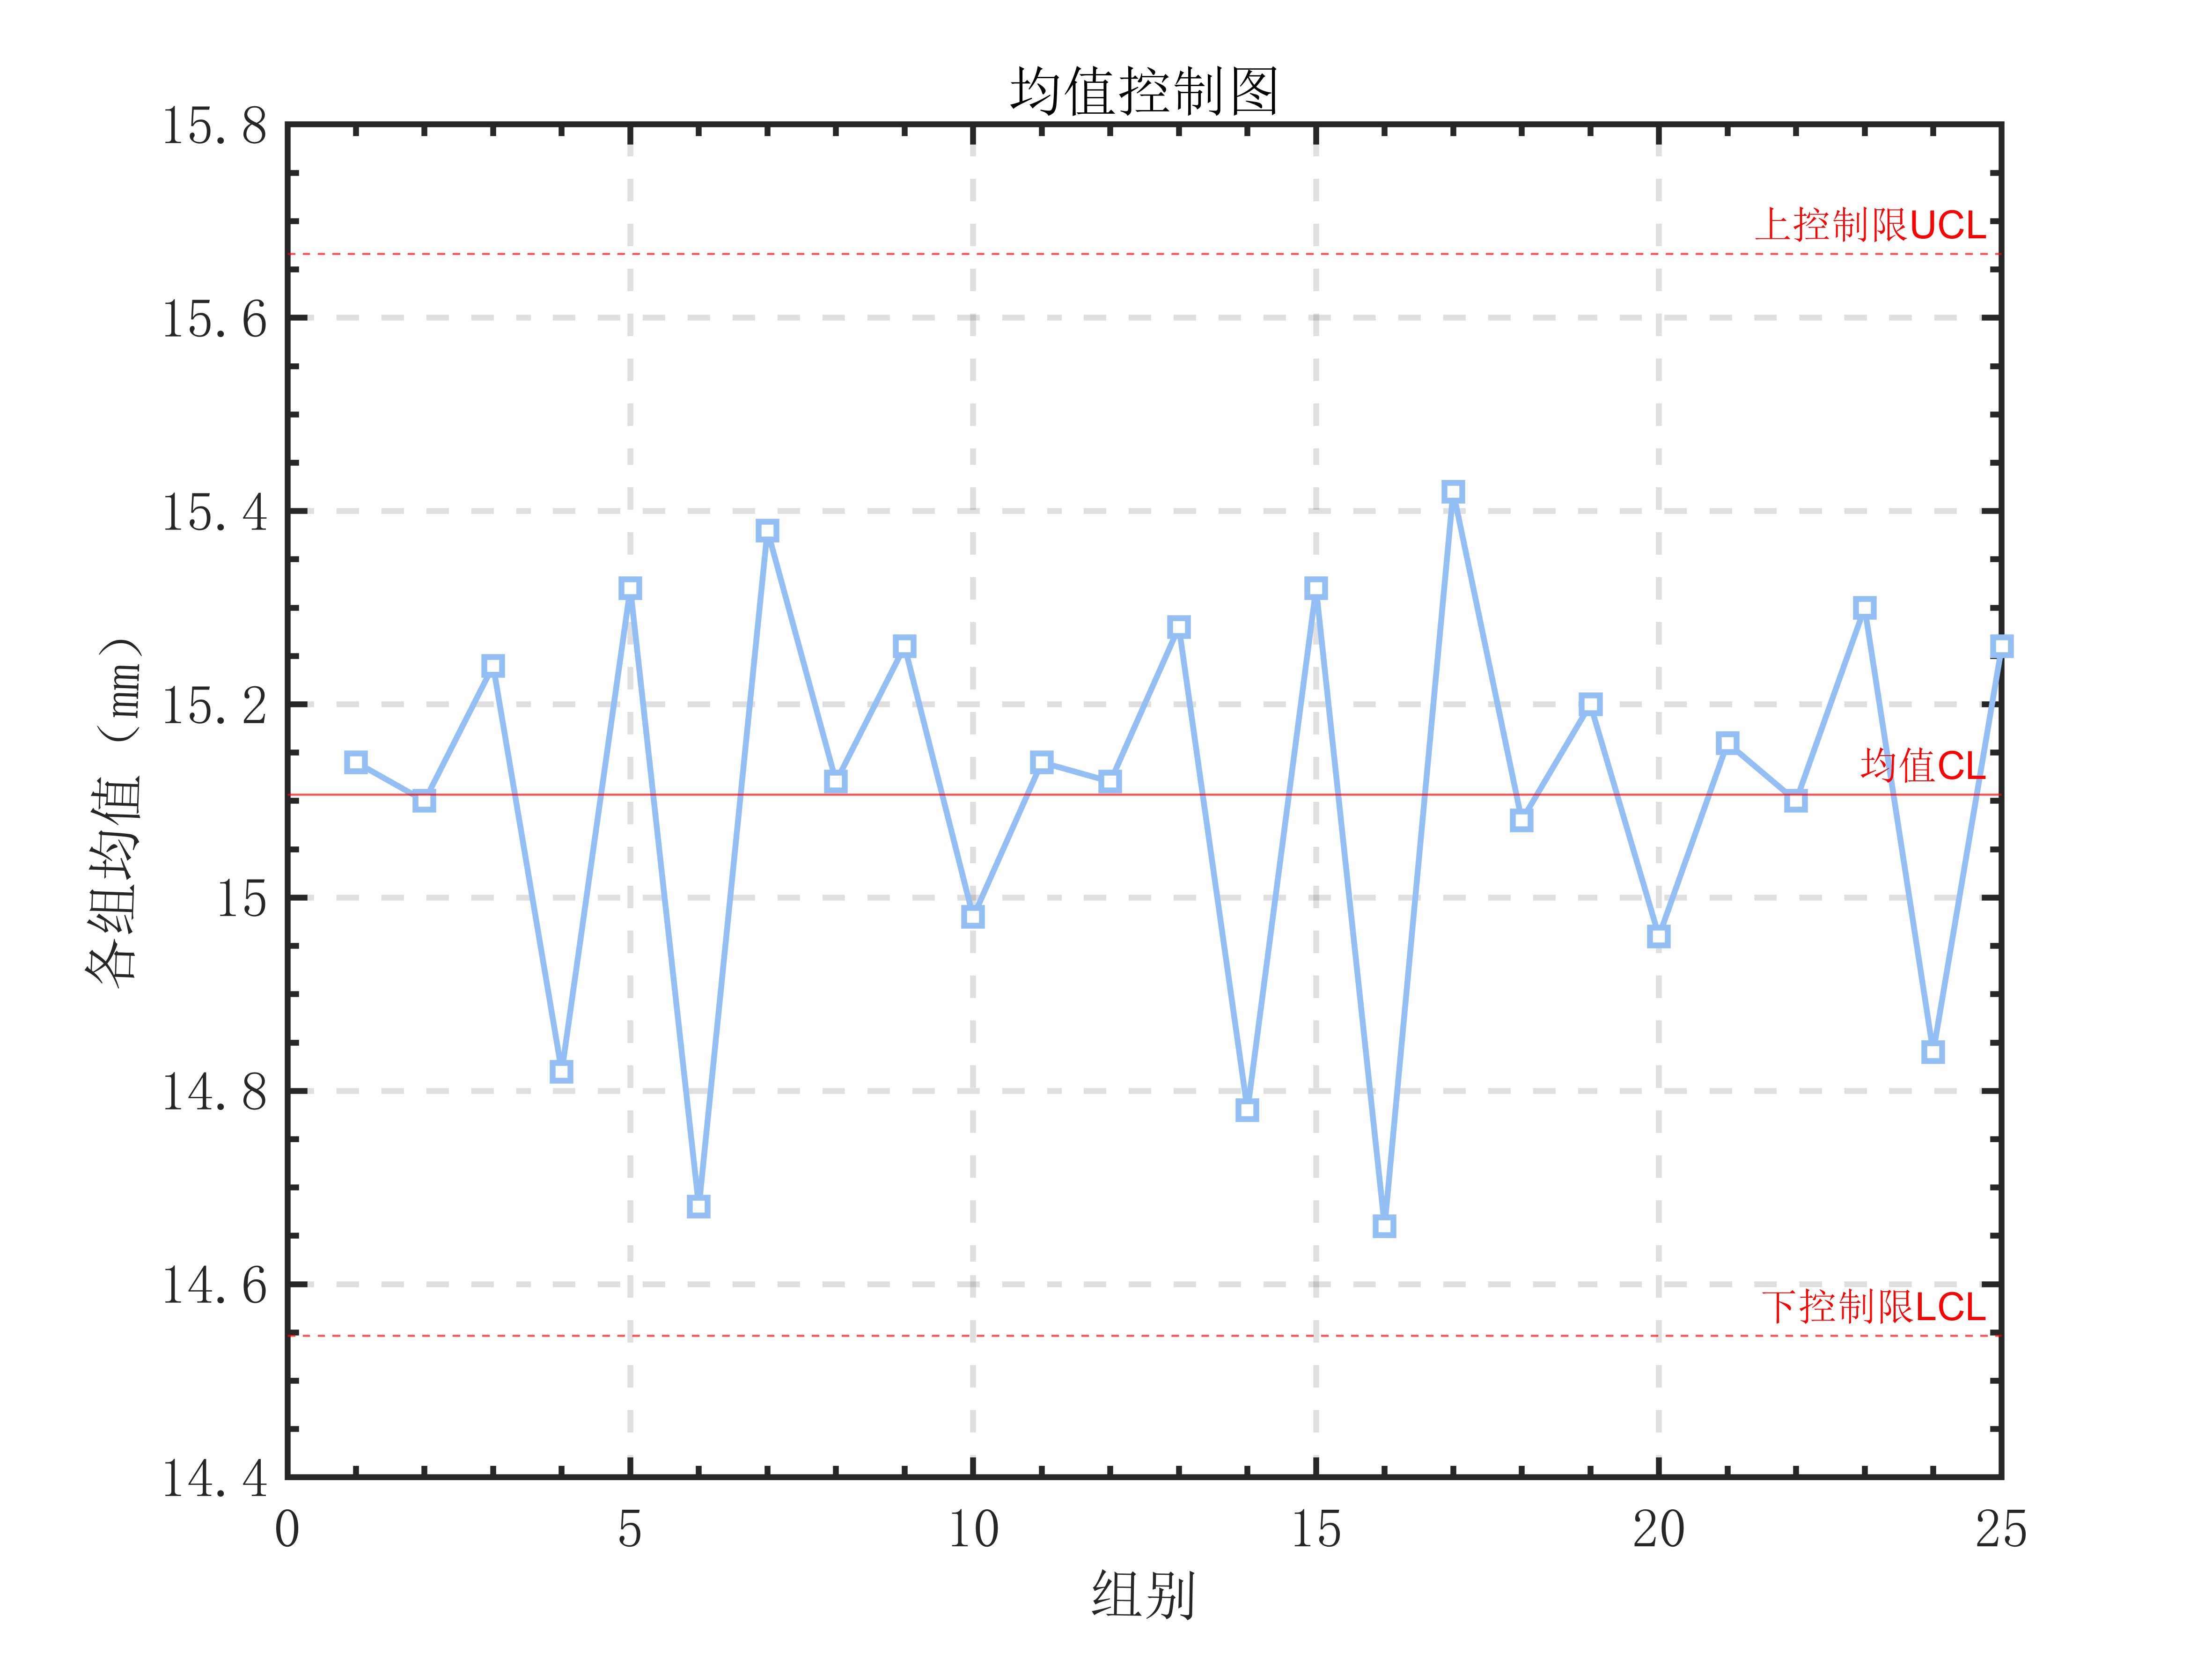
\includegraphics[width=0.8\textwidth]{2.png}
\end{figure}

但在实际生产实践中,并不是所有的产品工艺指标都会近似服从正态分布。因此,在实际操作中,均值控制限常用如下公式估算:

\begin{itemize}
	\setlength{\parsep}{0ex} %段落间距
	\setlength{\topsep}{2ex} %列表到上下文的垂直距离
	\setlength{\itemsep}{1ex} %条目间距
	\item $UCL=\hat{\mu}+A_s\bullet \hat{s}$
	\item $CL=\hat{\mu}$ 
	\item $LCL=\hat{\mu}-A_s\bullet \hat{s}$
\end{itemize}

其中,若采集工艺参数样本数据组数$k=25$,各批次数据数量$n=5$,令$x_{ij}$表示第$i$批次的第$j$个数据,$\bar{x_i}$表示组内均值;则可用$\mu$表示个各批次所有数据的样本均值,$\hat{s}$表示各个批次数据标准偏差的算数平均值,即:

\begin{equation}
	{\bar{x}}_i=\frac{1}{n}\sum_{j=1}^{n}x_{ij}
\end{equation}

\begin{equation}
	\hat{s}=\frac{1}{k}\sum_{i=1}^{k}{\hat{s}}_i
\end{equation}

\begin{equation}
\hat{\mu}=\frac{1}{k}\sum_{i=1}^{k}{\bar{x}}_i=\frac{1}{kn}\sum_{i=1}^{k}\sum_{j=1}^{n}x_{ij}
\end{equation}

\begin{equation}
	{\hat{s}}_i=\sqrt{\frac{1}{n-1}\sum_{j=1}^{n}{{(x}_{ij}-{\bar{x}}_i)}^2}
\end{equation}

又查表\upcite{2}可得:当每批次样本数据数$n=5$时,有$A_s=1.427$。

于是绘制出实际均值控制图:

\begin{lstlisting}
figure;
plot(means, 'o-');
xi=mean(data, 2);
for i=1:num_groups
	sum=0;
	for j=1:samples_per_group
		sum=sum+((data(i,j)-xi(i))^2);   
	end
	si_hat(i)=sqrt(sum/(num_groups-1));
end
s_hat=mean(si_hat);
As=1.427;
CL= miu_hat;
UCL=miu_hat+s_hat*As;
LCL=miu_hat-s_hat*As;
yline(CL, 'r-', 'CL');
yline(UCL, 'r--', 'UCL');
yline(LCL, 'r--', 'LCL');
\end{lstlisting}

\begin{figure}[H]
	\centering
	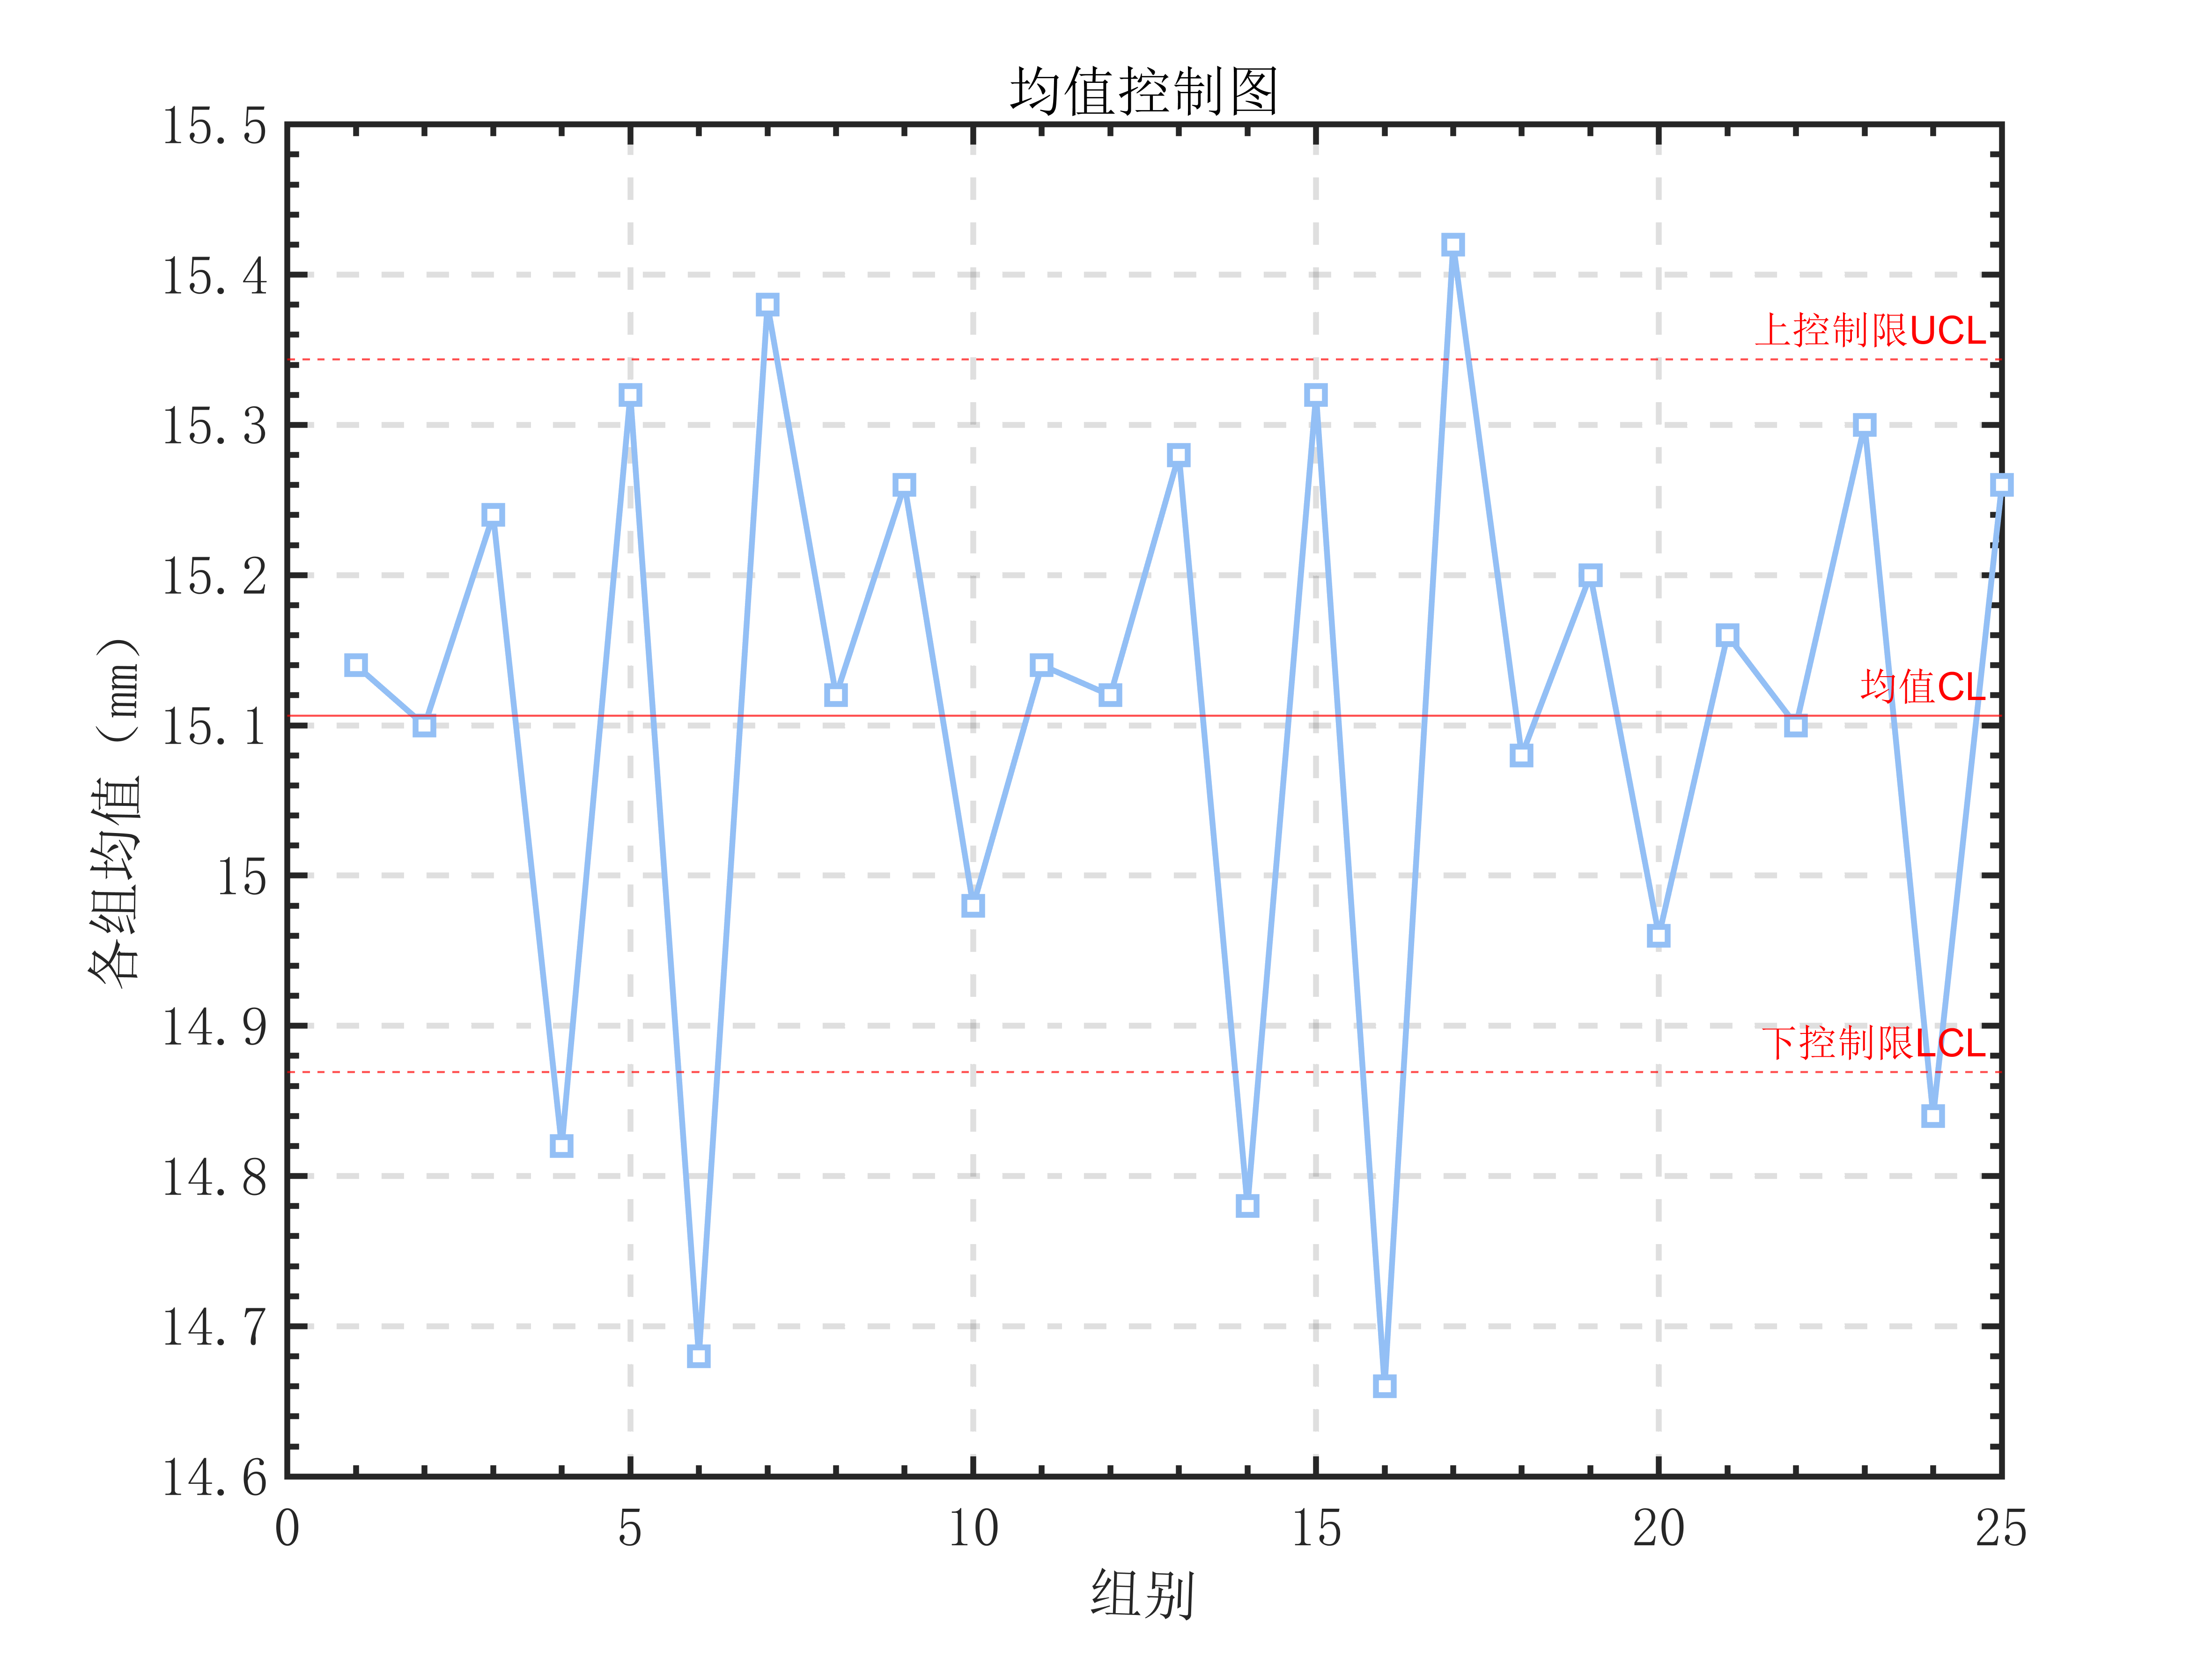
\includegraphics[width=0.8\textwidth]{3.png}
\end{figure}

\subsubsection{方差控制图}
方差控制图的结构与均值控制图非常类似,也是由中心线以及上下控制限构成。只是图中的数据点描述的每批次数据的标准偏差,因此可用于定量判断不同批次数据的标准偏差(数据的波动性)在变化中是否存在“异常因素”。

类似于均值控制图,在实际操作中,常用如下公式估算其中心线以及上下控制限: 
\begin{itemize}
	\setlength{\parsep}{0ex} %段落间距
	\setlength{\topsep}{2ex} %列表到上下文的垂直距离
	\setlength{\itemsep}{1ex} %条目间距
	\item $UCL=B_U\bullet\ \hat{s}$
	\item $CL=\hat{s}$ 
	\item $LCL=B_L\bullet\hat{s}$
\end{itemize}

其中$B_U$、$B_L$为依赖于每批次样本数据数$n$的常数参数,查表\upcite{2}可得:当每批次样本数据数$n=5$时,有$B_U=2.089$、$B_L=0$。

据此可绘制出对应的方差控制图:

\begin{lstlisting}
Bu=2.089;
Bl=0;
figure;
plot(variances, 'o-');
hold on;
UCL=(Bu*s_hat);
CL=(s_hat);
LCL=(Bl*s_hat);
yline(CL, 'r-', 'CL');
yline(UCL, 'r--', 'UCL');
yline(LCL, 'r--', 'LCL');
\end{lstlisting}

\begin{figure}[H]
	\centering
	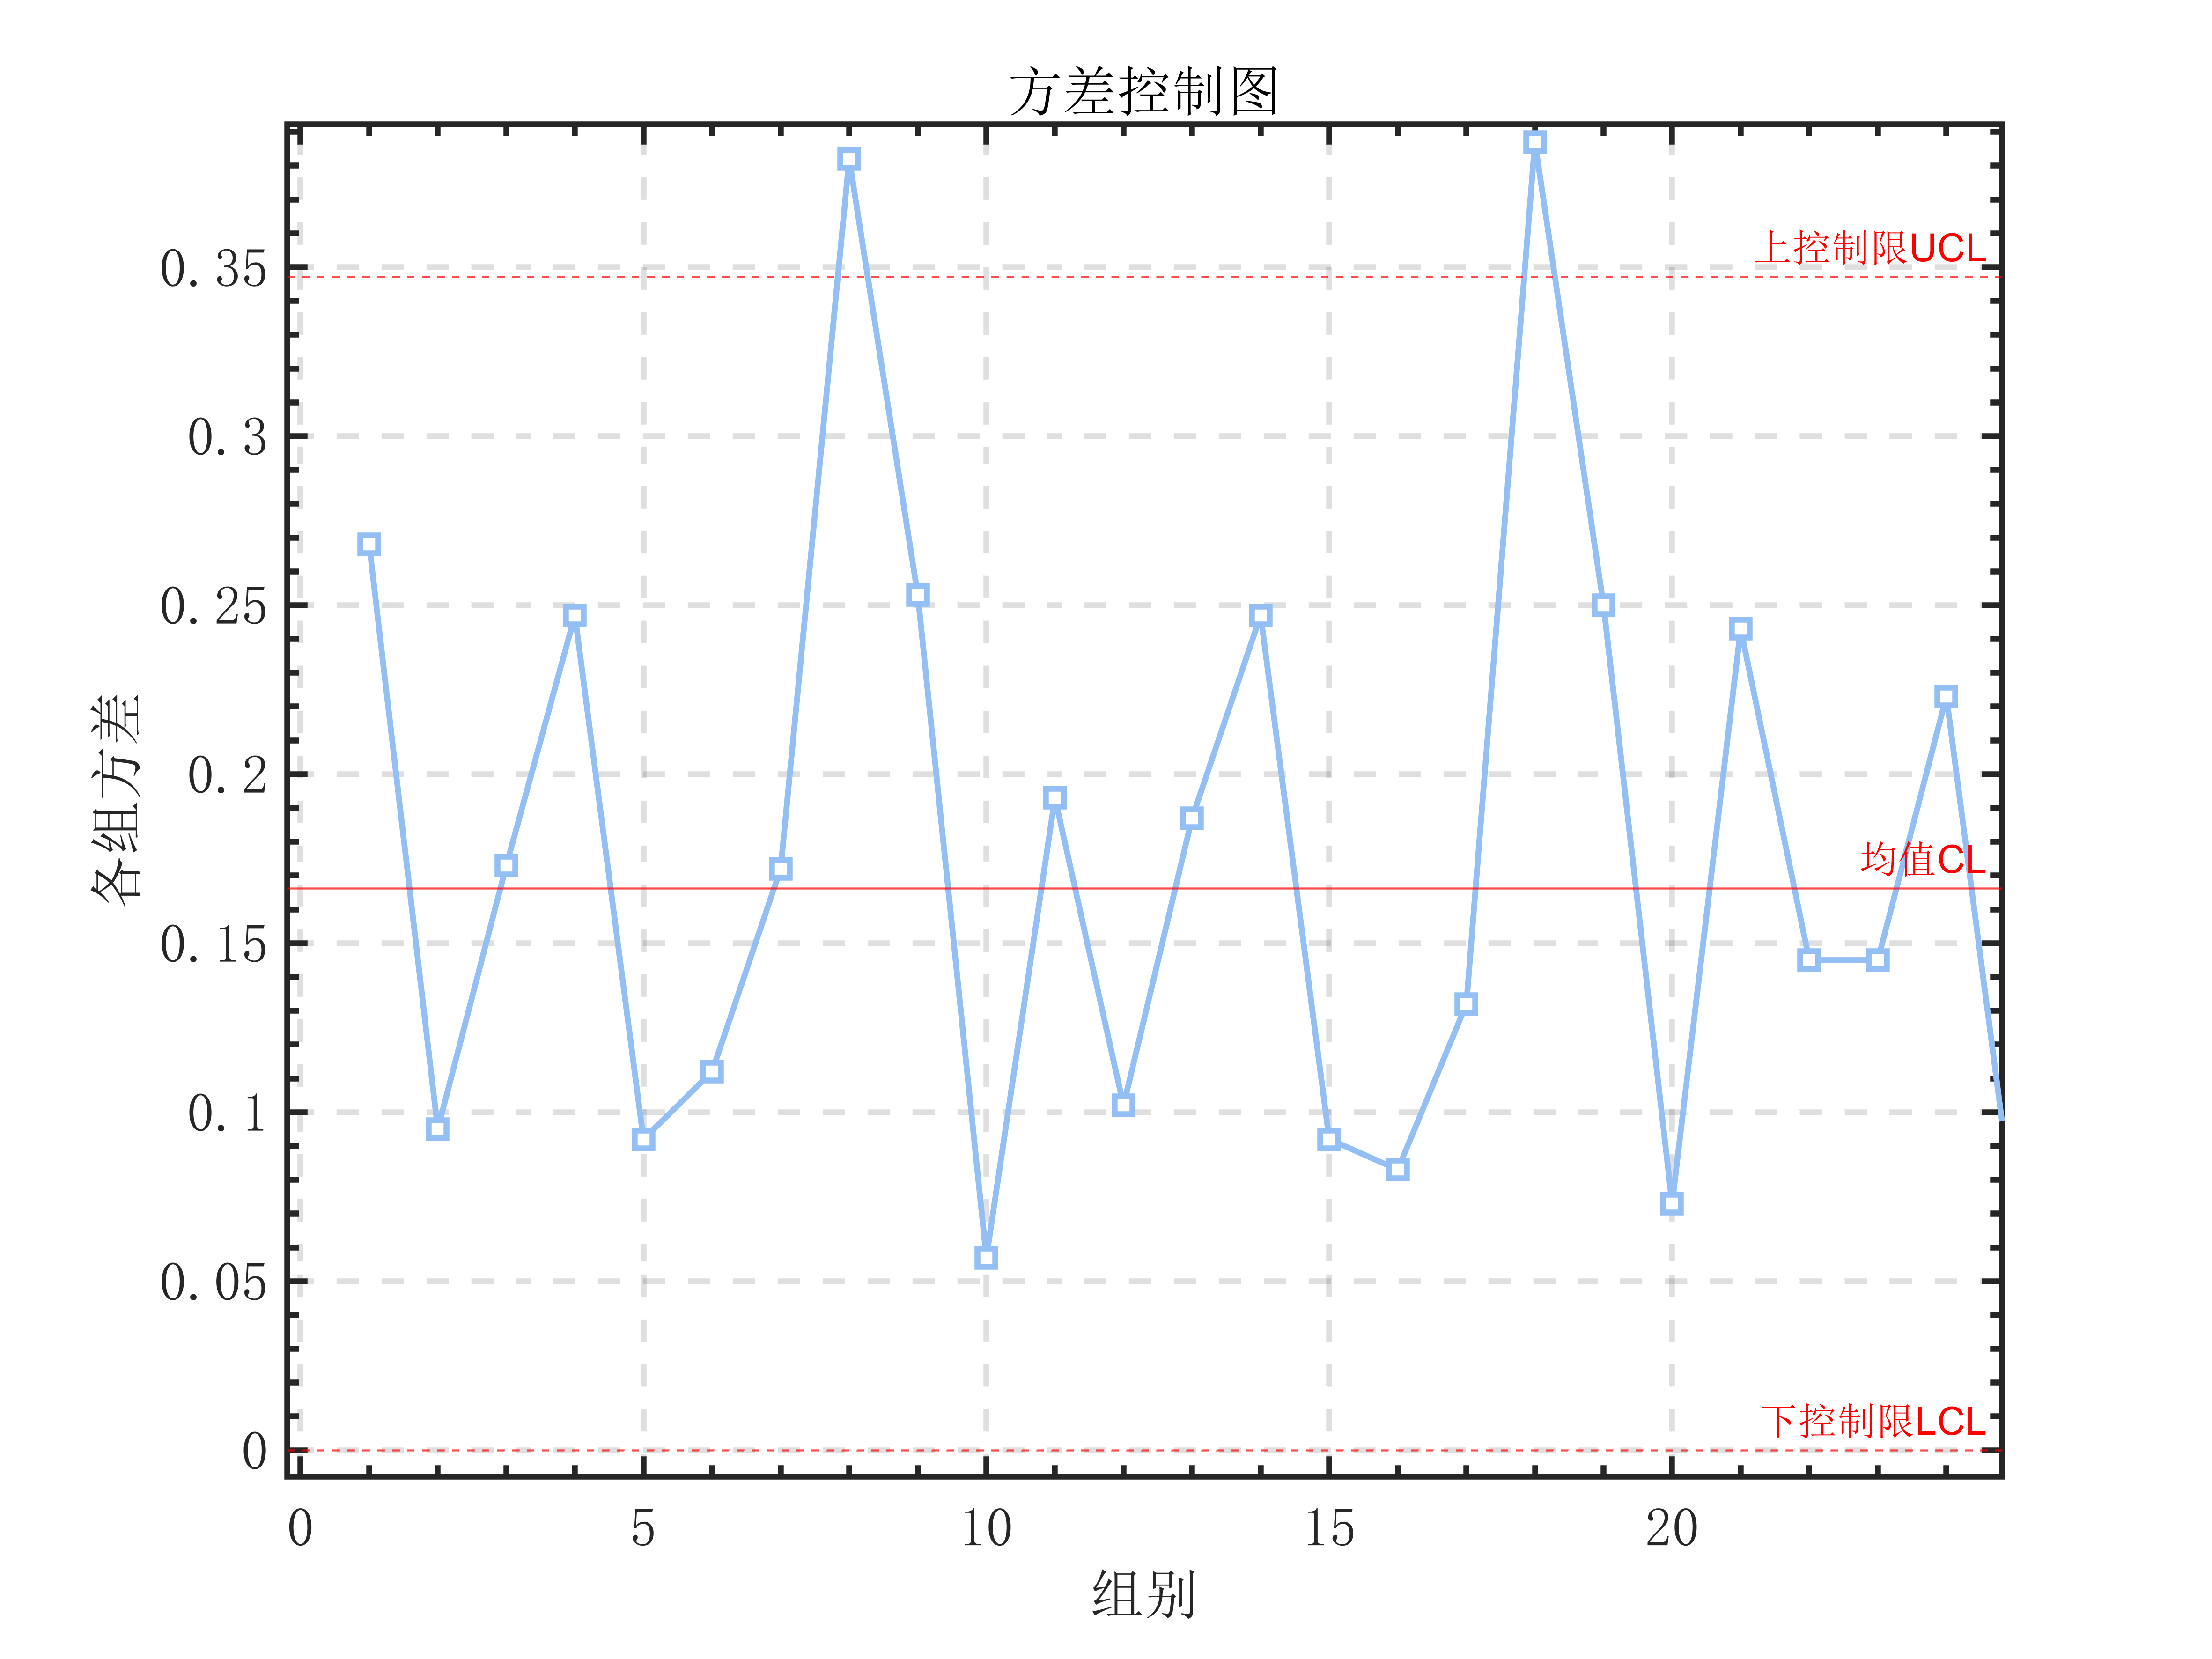
\includegraphics[width=0.8\textwidth]{4.png}
\end{figure}

\section{产品质量分析结论}	
为根据Shewhart控制图判断产品生产过程是否受控,可对于均值控制图与方差控制图分别采用如下八条常见规则(规则均不能触碰,否则视为不受控),以识别产品生产过程是否仅受到随机因素影响:

\begin{itemize}
	\setlength{\parsep}{0ex} %段落间距
	\setlength{\topsep}{2ex} %列表到上下文的垂直距离
	\setlength{\itemsep}{1ex} %条目间距
	\item \textbf{规则 1}:控制图上有一个点(对应某个批次数据)位于控制限以外;		
	\item \textbf{规则 2}:连续9个点落在中心线同一侧;
	\item \textbf{规则 3}:连续6个点递增或者递减;
	\item \textbf{规则 4}:连续14个点交替上下;
	\item \textbf{规则 5}:连续3个点中有2个点落在中心线同侧的B区以外;
	\item \textbf{规则 6}:连续5个点中有4个点落在中心线同侧的C区以外;
	\item \textbf{规则 7}:连续15个点落在中心线两侧的C区;
	\item \textbf{规则 8}:连续8个点落在中心线两侧且无一点在C区以内。
\end{itemize}

其中,A、B、C分区如下图\upcite{2}所示,C区为以CL控制限为对称轴的中心区域,B、A两区向两侧延伸至上下控制限UCL与LCL。

\begin{figure}[H]
	\centering
	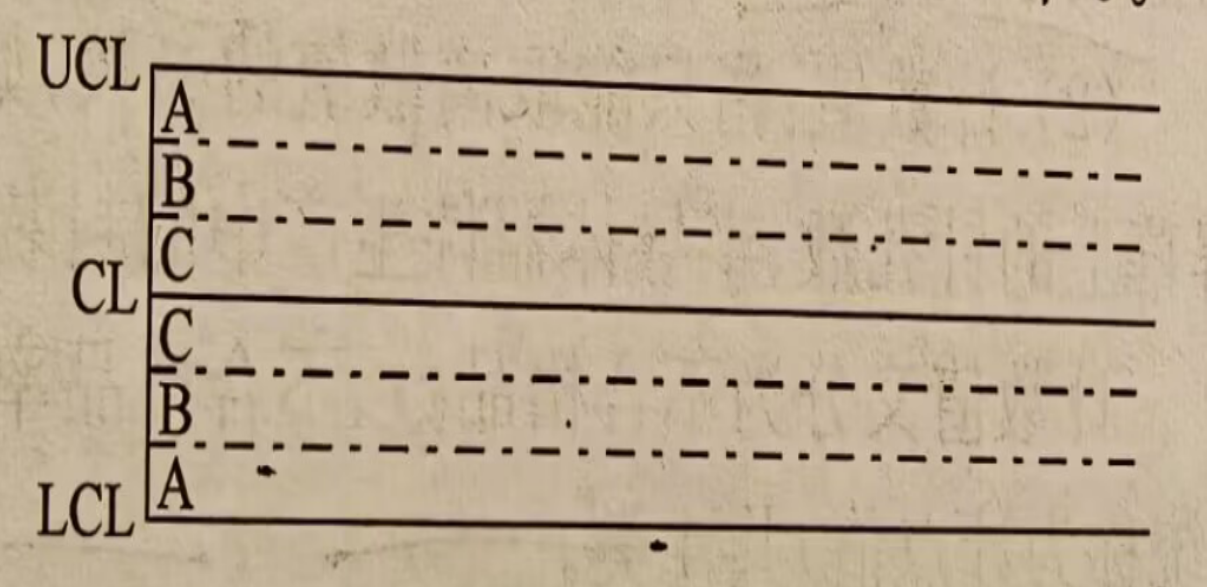
\includegraphics[width=0.8\textwidth]{5.png}
\end{figure}

实际上,Matlab软件中对于Shewhart控制图以及SPC统计过程控制方法有一套完整封装的库函数$controlchart()$,调用结果如下所示:

\begin{lstlisting}
load parts
[st,plotdata] = controlchart(data,'charttype',{'xbar' 's'});
\end{lstlisting}

\begin{figure}[H]
	\centering
	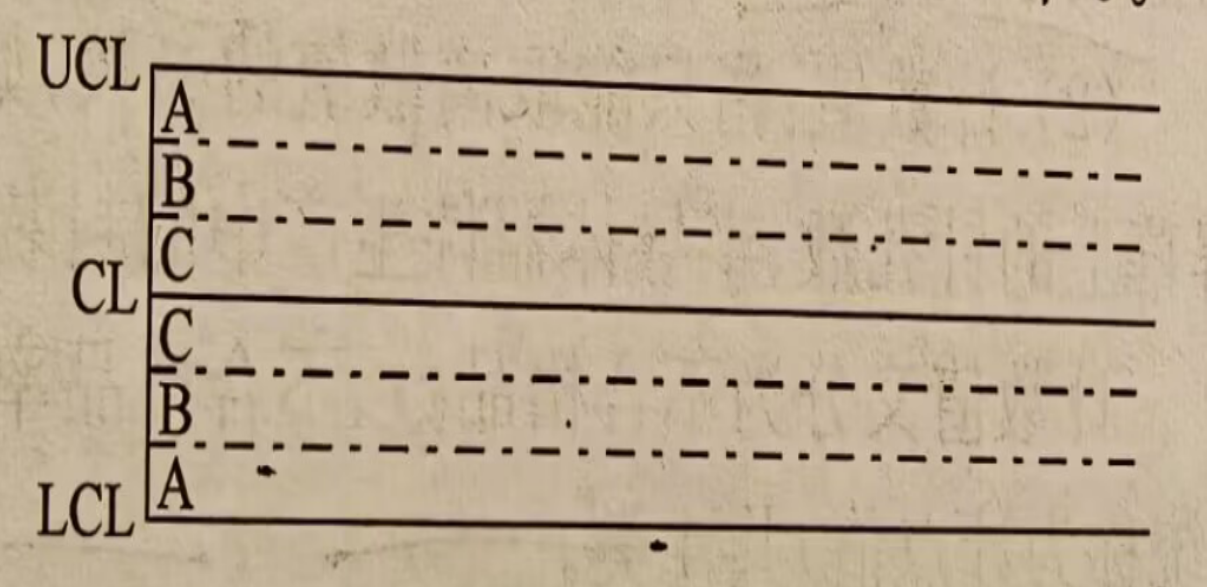
\includegraphics[width=0.8\textwidth]{5.png}
\end{figure}

其中第一张图为均值控制图,第二张图为标准差控制图。

通过观察图像,基于八大规则进行判断并通过查看返回对象$plotdata$的$ooc$属性(Logical that is true for points that are out of control)可知,\textbf{该产品生产过程确实处于统计受控状态}。除此之外,\textbf{样本均值也在15.1mm左右,符合对于滚珠直径的一般行业要求,工艺水平良好;但实际工序能力指数$Cpk$仅有0.6896,说明工艺水平还有上升空间}。

\begin{thebibliography}{99}
	\bibitem{1} 茆诗松,程依明,濮晓龙编著. 概率论与数理统计教程[M]. 高等教育出版社, 2019.
	\bibitem{2} 贾新章 .. [等] 编著. 统计过程控制理论与实践[M]. 电子工业出版社, 2017.
\end{thebibliography}

\end{document} 
